\chapter{Data Structures for Inverted Index}
In this chapter we will analyze which data structures are used for Inverted Index and a naive approach 
consist in save in a dictionary but this cause a waste in memory and not helps in retrieve elements quickly.

To improve exact and prefix search are usually used the following data structures:
\begin{itemize}
	\item Hashing
	\item Tree
	\item Trie, also called \emph{prefix tree}, is an ordered tree data structure used to store a dynamic set
	      or associative array where the keys are usually strings.\newline
	      All the descendants of a node have a common prefix of the string associated with that node,
	      and the root is associated with the empty string; keys tend to be associated with leaves,
	      though some inner nodes may correspond to keys of interest and hence, keys are not necessarily
	      associated with every node.

	      Solves the prefix problem, but has $O(p)$ time, with many cache misses and from $10$ to $60$ (or, even more) bytes per node.

\end{itemize}
To improve our search we exploits $2$-level caching indexing, that improve search, typically $1$ I/O $+$ in-mem comparison and 
improve also space requirement, because we use a trie built over a subset of string and front-coding over buckets.\newline
A disadvantage is the trade-off between speed and space, caused by bucket size.

Front-coding is a type of delta encoding compression algorithm whereby common prefixes or suffixes and their lengths 
are recorded so that they need not be duplicated and this algorithm is particularly well-suited for compressing sorted data,
as we can see in figure \ref{img:front-coding}.

\begin{figure}
	\caption{Example of Front Coding}
	\label{img:front-coding}
	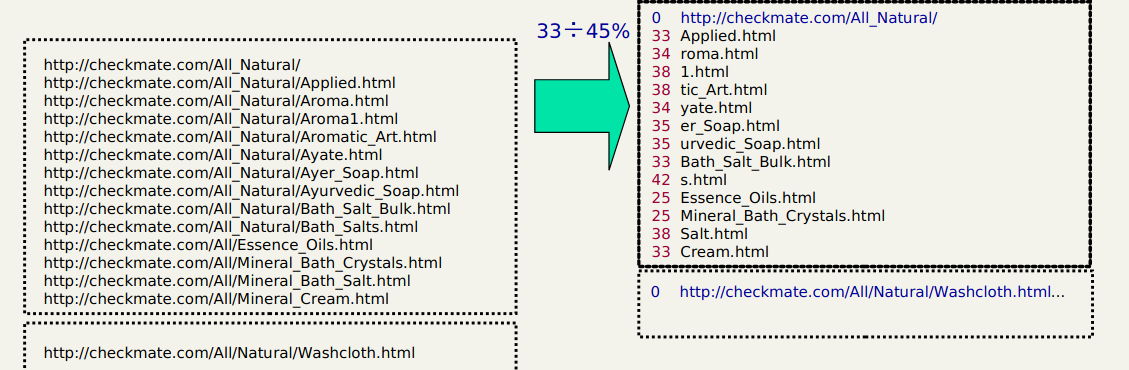
\includegraphics[width=\textwidth]{Images/frontCoding}
\end{figure}

\section{Correction Queries}
Spell correction has $2$ principal uses:
\begin{enumerate}
    \item Correcting document(s) to be indexed.
    \item Correcting queries to retrieve “right” answers.
\end{enumerate}
There are two approaches that can be used:
\begin{enumerate}
    \item Isolated word: check each word on its own for misspelling.
    \item Context-sensitive is more effective and look at surrounding words.
\end{enumerate}
To correct isolated word there is a lexicon from which the correct spellings come and two basic choices for this are
a standard lexicon such as Webster’s English Dictionary or an “industry-specific” lexicon, that is specific for a field and where
we can use mining algorithms to derive possible corrections.

Isolated word correction consist that given a lexicon and a character sequence $Q$, return the words in the lexicon closest
to $Q$; for estabilish what's closest we will study several measures (we will study Edit distance, Weighted edit distance and
$n$-gram overlap).

Edit Distance is generally found by dynamic programming and consist given two strings $S1$ and $S2$, to find the minimum number of 
operations to convert one to the other (Operations are typically character-level insert, delete, replace, with possibility of also transposition.

In figure \ref{img:editDistance} is possible to find how is computed the edit distance and we compute the table of distance from 
bottom to top, using equation described in the figure.

\begin{figure}
	\caption{Equation for computing Edit Distance}
	\label{img:editDistance}
	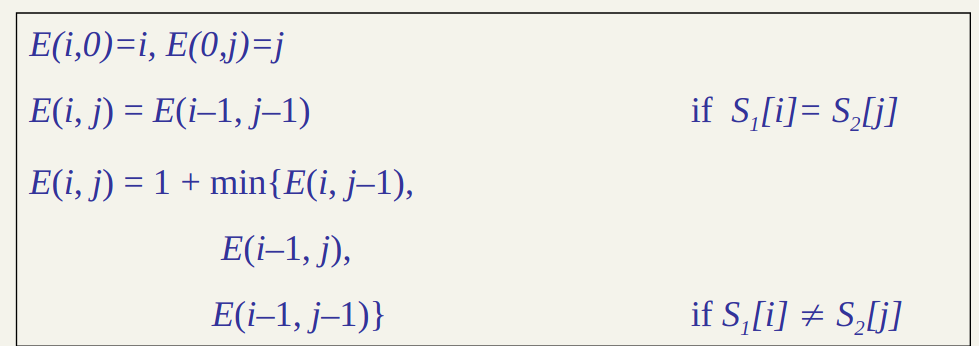
\includegraphics[width=\textwidth]{Images/editDistance}
\end{figure}
We introduce now \emph{Weighted edit distance}, where the weight of an operation depends on the character(s) involved and 
meant to capture keyboard errors, as for example $m$ is more likely to be mis-typed as $n$ than as $q$.\newline
Therefore, replacing $m$ by $n$ is a smaller cost than by $q$ and requires weighted matrix as input.

We create two dictionaries $D_1 = \{ strings \}$ and $D_2 = \{ strings of D1 with one deletion \}$; for a query we have to 
do 1 search in $D_1$ in perfect match, $1$ query in $D_2$ to find $1$-char less, $p$ queries to find $P$ with $1$-char less from $D_2$ to $D_1$
and in the end $p$ queries to find substitution in $D_2$ from $P$ with $1$-char less.

We need $2p + 2$ hash computations for $P$ and the positive aspects are that is CPU efficient, no cache misses for computing P’s hashes,
but $O(p)$ cache misses to search in $D_1$ and $D_2$, instead negative aspects are large space because of the many strings in $D_2$ 
which must be stored to search in the hash table of D2, unless we avoid collision and the presence of false matches.

A better approach consist to use overlap distance, where we use the $k$-gram index contains for every $k$-gram all terms including
that $k$-gram and we append $k-1$ symbol \$ at the front of each string, in order to generate a number $L$ of $k$-grams 
for a string of length $L$

We select terms by threshold on matching $k$-grams and if the term is $L$ chars long (it consists of $L k$-grams) and if $E$
is the number of allowed errors ($E*k$ of the $k$-grams of $Q$ might be different from term’s ones because of the $E$ errors) and 
so at least $L – E*k$ of the $k$-grams in $Q$ must match a dictionary term to be a candidate answer and if ED is required,
post-filter results with dynamic programming.

We enumerate multiple alternatives and then need to figure out which to present to the user for “Did you mean?" and we use heuristics:
the alternative hitting most docs and query log analysis + tweaking (done for especially popular, topical queries), anyway
spell-correction is computationally expensive and is run only on queries that matched few docs.

We introduce now how to deal with \emph{wildcard queries} and to deal we use \emph{permuterm index}, where we have the 
following possible queries:
\begin{itemize}
    \item X lookup on X\$
    \item X* lookup on   \$X*
    \item *X lookup on X\$*
    \item *X* lookup on X*
    \item X*Y lookup on Y\$X*
\end{itemize}
The permuterm query processing consist to rotate query wild-card to the right so P*Q become Q\$P* so now we 
use prefix-search data structure and a problem of Permuterm is that has $\approx 4x$ lexicon size (an empirical observation for English).

\emph{Soundex} is a class of heuristics to expand a query into phonetic equivalents, it is language specific used mainly for names
and was invented for the U.S. census in 1918.\newline
We introduce now the original algorithm that consist to turn every token to be indexed into a reduced form consisting of $4$ chars
and do the same with query terms, so we build and search an index on the reduced forms (in figure \ref{img:soundex} are indicated
all steps of basic algorithm).

\begin{figure}
	\caption{Soundex basic Algorithm}
	\label{img:soundex}
	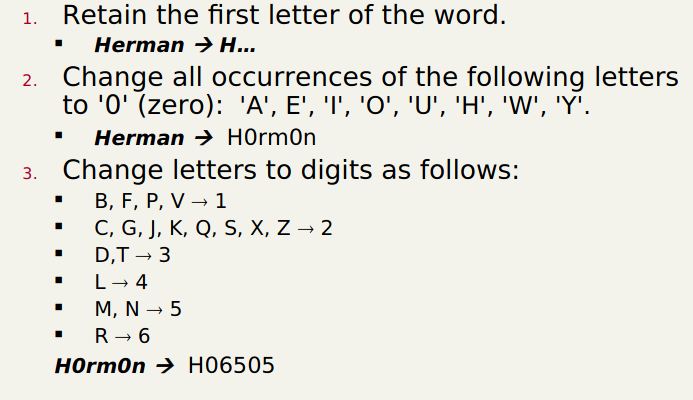
\includegraphics[width=\textwidth]{Images/soundex1}
	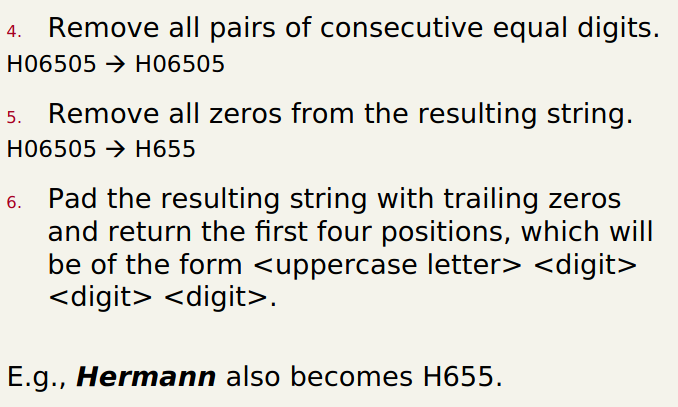
\includegraphics[width=\textwidth]{Images/soundex2}
\end{figure}
Soundex is the classic algorithm, provided by most databases (Oracle, Microsoft, and so on) but is not very useful for information retrieval;
is okay for “high recall” tasks (e.g., Interpol), though biased to names of certain nationalities, so other algorithms
for phonetic matching perform much better in the context of IR.


